\section{Circuits and Hardware Description Languages}

  We have seen in our theoretical computer science that the $\NAND$ gate is univeral, and we have implemented it with transistors in the previous chapter. Therefore using syntactic sugar, we can apply the rest of the elementary gates. The common unary and binary logic gates are listed below as a refresher. 

  \begin{figure}[H]
    \centering 
    \begin{subfigure}[b]{0.32\textwidth}
      \centering
      \begin{tikzpicture}[circuit logic US]
        \node[and gate, draw, logic gate inputs=nn] (A) at (0,0) {};
        \node[above=0.3cm of A] {AND};
        \draw (A.input 1) -- ++(-0.5,0);
        \draw (A.input 2) -- ++(-0.5,0);
        \draw (A.output) -- ++(0.5,0);
      \end{tikzpicture}
      \caption{AND Gate}
      \label{fig:and}
    \end{subfigure}
    \hfill 
    \begin{subfigure}[b]{0.32\textwidth}
      \centering
      \begin{tikzpicture}[circuit logic US]
        \node[or gate, draw, logic gate inputs=nn] (O) at (0,0) {};
        \node[above=0.3cm of O] {OR};
        \draw (O.input 1) -- ++(-0.5,0);
        \draw (O.input 2) -- ++(-0.5,0);
        \draw (O.output) -- ++(0.5,0);
      \end{tikzpicture}
      \caption{OR Gate}
      \label{fig:or}
    \end{subfigure}
    \hfill 
    \begin{subfigure}[b]{0.32\textwidth}
      \centering
      \begin{tikzpicture}[circuit logic US]
        \node[not gate, draw] (N) at (0,0) {};
        \node[above=0.3cm of N] {NOT};
        \draw (N.input) -- ++(-0.5,0);
        \draw (N.output) -- ++(0.5,0);
      \end{tikzpicture}
      \caption{NOT Gate}
      \label{fig:not}
    \end{subfigure}
    
    \begin{subfigure}[b]{0.32\textwidth}
      \centering
      \begin{tikzpicture}[circuit logic US]
        \node[nand gate, draw, logic gate inputs=nn] (AN) at (0,0) {};
        \node[above=0.3cm of AN] {NAND};
        \draw (AN.input 1) -- ++(-0.5,0);
        \draw (AN.input 2) -- ++(-0.5,0);
        \draw (AN.output) -- ++(0.5,0);
      \end{tikzpicture}
      \caption{NAND Gate}
      \label{fig:nand}
    \end{subfigure}
    \hfill 
    \begin{subfigure}[b]{0.32\textwidth}
      \centering
      \begin{tikzpicture}[circuit logic US]
        \node[nor gate, draw, logic gate inputs=nn] (NO) at (0,0) {};
        \node[above=0.3cm of NO] {NOR};
        \draw (NO.input 1) -- ++(-0.5,0);
        \draw (NO.input 2) -- ++(-0.5,0);
        \draw (NO.output) -- ++(0.5,0);
      \end{tikzpicture}
      \caption{NOR Gate}
      \label{fig:nor}
    \end{subfigure}
    \hfill 
    \begin{subfigure}[b]{0.32\textwidth}
      \centering
      \begin{tikzpicture}[circuit logic US]
        \node[xor gate, draw, logic gate inputs=nn] (X) at (0,0) {};
        \node[above=0.3cm of X] {XOR};
        \draw (X.input 1) -- ++(-0.5,0);
        \draw (X.input 2) -- ++(-0.5,0);
        \draw (X.output) -- ++(0.5,0);
      \end{tikzpicture}
      \caption{XOR Gate}
      \label{fig:xor}
    \end{subfigure}
    \caption{Common Logic Gates}
    \label{fig:logic-gates}    
  \end{figure}

  Now that we know about chips, perhaps we are ready to mass produce them. Consider the following scenario where you are a hardware engineer with three boxes full of $\AND, \OR, \NOT$ gates. You need to ship an order of 1000 $\XOR$ gates. How would you do this? To construct one $\XOR$ gate, you can follow the example below. 

  \begin{figure}[H]
    \centering 
    \begin{tikzpicture}[circuit logic US]
      % Input nodes
      \node (a) at (0,3) {a};
      \node (b) at (0,1) {b};

      % NOT gates (top and bottom)
      \node[not gate, draw] (not1) at (2,2.5) {};
      \node[not gate, draw] (not2) at (2,1.5) {};

      % AND gates
      \node[and gate, draw] (and1) at (5,2.9) {};
      \node[and gate, draw] (and2) at (5,1.1) {};

      % OR gate
      \node[or gate, draw, logic gate inputs=nn] (or1) at (6,2) {};

      % Output node
      \node (out) at (7,2) {out};

      % Main input lines with junction dots
      \draw (a) -- (1,3) node[circle,fill,inner sep=1pt] {} -- (1.5,3);
      \draw (b) -- (1/5,1) node[circle,fill,inner sep=1pt] {} -- (1.5,1);

      % Connections from input a
      \draw (1,3) |- (not2.input);
      \draw (1,3) -- (3.5,3) |- (and1.input 1);

      % Connections from input b  
      \draw (1.5,1) |- (not1.input);
      \draw (1.5,1) -- (3.5,1) |- (and2.input 2);

      % NOT gate outputs to AND gates
      \draw (not1.output) |- (and1.input 2);
      \draw (not2.output) |- (and2.input 1);

      % AND gate outputs to OR gate with junction dots
      \draw (and1.output) |- (or1.input 1);
      \draw (and2.output) |- (or1.input 2);

      % Final output
      \draw (or1.output) -- (out);
    \end{tikzpicture}
    \caption{XOR Chip from AON gates.} 
    \label{fig:xor_from_aon}
  \end{figure}

  We would take two $\AND$ gates, two $\NOT$ gates, and one $\OR$ gate, mount them on a board according to the figure's layout, and connect the chips to one another by running copper wires among them and soldering the wire ends to the respective input/output pins. After this, we will have 3 exposed wire ends---two inputs and one output. We then solder a pin to each one of these wire ends, seal the entire device (except for the three pins) in a plastic encasing, and label it as $\XOR$. Do this 1000 times and you're done. 

  There's a lot of problems with this, with the foremost being that this might be error-prone, especially in more complex chips. There is guarantee that the given chip diagram is correct. Although we can prove correctness in simple cases like $\XOR$, we cannot do so in realistically complex chips. Thus, we need to empirically test the chip, i.e. connect it to a power supply, activate/deactivate the input pins in various configurations, and hope that the chip outputs will agree with its specifications. 

  Even this debugging process can be quite time-intensive if we endlessly tinker with wires and circuits. Therefore, engineers simulate the construction and testings of these circuits with \textbf{hardware simulators}. Remember that we have established that \textit{straight-line programs} are an equivalent model of finite computation, and so we can use lexical programs to model boolean circuits. These programs are called \textbf{hardware description languages (HDL)} (analogous to software language) and are used to model and design these digital systems. Once you have written a script in some HDL, you can use a \textbf{hardware simulator} (analogous to compiler) to test the circuit. We will use the Verilog language along with the Icarus Verilog hardware simulator.\footnote{Historically the \textit{VHDL} language was created as a military project---and is still in use---but is a bit ugly.  Then, \textit{Verilog} became the most dominant, but it has been largely replaced by \textit{SystemVerilog}. Regardless, both of these are a superset of Verilog, and we will begin with this. Given the Verilog language, \textit{Icarus Verilog} is its corresponding open-source hardware simulator that runs on all platforms (Windows, Mac, Linux).}

  \begin{definition}[Module]
    A \textbf{module} represents some sort of class. 
    \begin{enumerate}
      \item \textbf{Ports} represent the inputs and outputs of a gate, represented with the \texttt{input} and \texttt{output} keywords. You might see a convention to put the outputs first and then the inputs. 
      \item \textbf{Wires} are used for connecting different elements, like physical wires between gates. You can think of them as signals, which can be read (is current flowing?) or assigned, but no values get stored in them. They are automatically updated when input changes are specified with the \texttt{wire} keyword. 
      \item \textbf{Regs} are like variables that store values---similar to physical registers in CPUs. They are specified with the \texttt{reg} keyword. 
      \item The output value is determined by some logic using the \texttt{assign} keyword. 
    \end{enumerate}
  \end{definition}

\subsection{Structural Modeling}

  There are two paradigms of writing Verilog. 
  
  \begin{definition}[Function Module]
    \begin{lstlisting}
      module nand_gate(
        input a, b,
        output y
      );
        assign y = ~(a & b);
      endmodule 
    \end{lstlisting}
  \end{definition}

  \begin{example}[Gate Level Implementation of Multiplexor]
    \begin{lstlisting}
      module multiplex_gate(A, B, X, out1); 
        input A, B, X; 
        output out1; 

        wire not_x; 
        wire out_and1, out_and2; 

        not not1(not_X, X); 
        and and1(out_and1, not_X, A); 
        and and2(out_and2, X, B); 
        or or1(out1, out_and1, out_and2); 
      endmodule
    \end{lstlisting}
  \end{example}

  Another way we can do this is by focusing on the flow of data. 

  \begin{example}[Dataflow Level Implementation of Multiplexor]
    \begin{lstlisting}
      module multiplex_gatel(A, B, X, out1); 
        input A, B, X; 
        output out1; 

        assign out1 = (~X&A)|(B&X);
      endmodule
    \end{lstlisting}
  \end{example}

\subsection{Behavioral Modeling}

  Can be efficient but a bit cryptic. So we really want to describe the behavior of the circuit rather than what the circuit actually is. So we do not have to worry about the implementation details, like an abstraction above the circuit. 

  \begin{example}[Behavioral Level Implementation of Multiplexor]
    In here, we don't care what the circuit looks like, and we model the behavior. 
    \begin{lstlisting}
      module multiplex_gate_level(A, B, X, out1); 
        input A, B, X; 
        output out1; 

        always @(*)
        begin
          if(X==0) 
            out1 = A; 
          else 
            out1 = B; 
        end
      endmodule
    \end{lstlisting}
  \end{example}

  \begin{definition}[Test Bench Module]
    A \textbf{testbench module} represents a suite of inputs that you want to test. The \textbf{device under test (dut)} connects the testbench signals to the DUT ports using named port connections. 

    \begin{lstlisting}[language=Verilog]
      module nand_gate_tb;
        reg a, b; // registers that hold states
        wire y;

        // Instantiate device under test
        nand_gate dut(.a(a), .b(b), .y(y));

        initial begin
          // Enable waveform dumping
          $dumpfile("nand_gate.vcd");
          $dumpvars(0, nand_gate_tb);

          // Test all input combinations
          a = 0; b = 0; #10;
          a = 0; b = 1; #10;
          a = 1; b = 0; #10;
          a = 1; b = 1; #10;

          $display("Test complete");
          $finish;
        end

        // Monitor changes
        initial
          $monitor("At time %t: a=%b, b=%b, y=%b", $time, a, b, y);
      endmodule
    \end{lstlisting}
  \end{definition}

\subsection{Test Benching}

  We've seen how to construct certain gates/chips in Verilog, but we don't know if the circuits actually do what we want. For this, we need to set up \textit{test bench modules}. With these, we can select a predetermined set of inputs and test the signals through each intermediate wire and the output for each. 

  \begin{example}[Test Benching Multiplexor]
    Here we show a testbench module that takes a predetermined set of inputs (all 8) and shows the signals traveling through each wire. 

    \begin{figure}[H]
      \centering 
      \begin{lstlisting}
        module tb_multiplex;
          reg A, B, X;
          wire out1;

          multiplex_gate uut(A, B, X, out1);

          initial begin
            // Test all combinations
            A = 0; B = 0; X = 0; #10;
            A = 0; B = 1; X = 0; #10;
            A = 1; B = 0; X = 0; #10;
            A = 1; B = 1; X = 0; #10;
            A = 0; B = 0; X = 1; #10;
            A = 0; B = 1; X = 1; #10;
            A = 1; B = 0; X = 1; #10;
            A = 1; B = 1; X = 1; #10;
            $finish;
          end

          initial begin
            $dumpfile("waves.vcd");
            $dumpvars(0, tb_multiplex);
          end
        endmodule
      \end{lstlisting}
      \caption{Test bench module for multiplexor in GTKwave.} 
    \end{figure}

    \begin{figure}[H]
      \centering 
      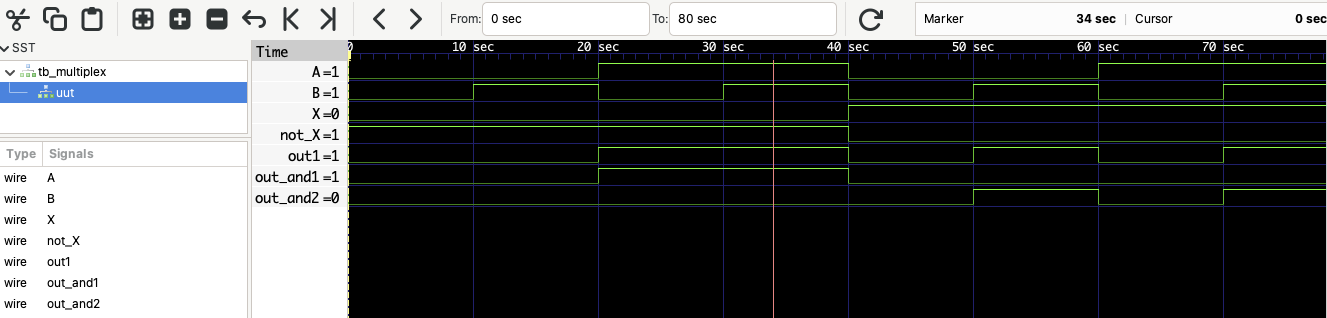
\includegraphics[scale=0.3]{img/multiplexor_gtk.png}
      \caption{View in GTKwave. You want to take a signal name in the bottom left and add it to the viewer by either double clicking on it or clicking ``append.''}
    \end{figure}
  \end{example}

\subsection{Multi-Bit Gates}

  \begin{definition}[Multi-Bit NOT Gate]
    
  \end{definition}

  \begin{definition}[Multi-Bit AND Gate]
    
  \end{definition}

  \begin{definition}[Multi-Bit OR Gate]
    
  \end{definition}

  \begin{definition}[Multi-Bit NAND Gate]
    
  \end{definition}

  \begin{definition}[Multi-Bit XOR Gate]
    
  \end{definition}

  \begin{definition}[Multi-Bit Multiplexor Gate]
    
  \end{definition}

  \begin{definition}[Multi-Bit Demultiplexor Gate]
    
  \end{definition}


